\documentclass[10pt, letterpaper]{article}
\usepackage[utf8]{inputenc}
\usepackage[english]{babel}

\usepackage{amsmath, amsfonts, amsmath, amssymb}
\usepackage{geometry}

\usepackage{tikz}
\usetikzlibrary{automata,positioning}

\usepackage{graphicx}
\usepackage{subcaption}
\usepackage{float}

\usepackage{hyperref} % Hyper-referencing within paper.

\usepackage[ruled, vlined, linesnumbered]{algorithm2e} % Used for pseudo-code
\usepackage{listings} % Used for including source code at the end.


% Commands go here.
\newcommand{\bx}{\boldsymbol x} % bold x
\newcommand{\R}{\mathbb{R}} % real numbers

\newcommand{\cov}{\boldsymbol \Sigma}
\newcommand{\scov}{\boldsymbol \sigma}
\newcommand{\sscov}{\sigma}

\newcommand{\preci}{\boldsymbol \Theta}
\newcommand{\spreci}{\boldsymbol \theta} % vector theta_{12}
\newcommand{\sspreci}{\theta} % point theta_{22}

\newcommand{\mean}{\boldsymbol \mu}
\newcommand{\iid}{\stackrel{\mathrm{i.i.d.}}{\sim}}
\newcommand{\tr}[1]{\mathrm{tr}\left[  #1 \right]}
\newcommand{\sampcov}{\boldsymbol S} % sample covariance S
\newcommand{\ssampcov}{\boldsymbol s}
\newcommand{\dualvar}{\boldsymbol Y} % dual variable
\newcommand{\sgn}[1]{\mathrm{sgn}\left( #1 \right) }

\newcommand{\eye}{\boldsymbol I} % identity matrix
\newcommand{\bzero}{{\bf 0}}
\newcommand{\bW}{\boldsymbol W}
\newcommand{\bZ}{\boldsymbol Z} % Z matrix for ADMM

\newcommand{\bsgn}{\boldsymbol \Gamma} % bold matrix of entry-wise signs
\newcommand{\bg}{\boldsymbol \gamma}
\newcommand{\one}{\boldsymbol 1} % bold 1

\newcommand{\diag}[1]{\mathrm{diag}\left( #1 \right)}
\newcommand{\abs}[1]{\mathrm{abs}\left( #1 \right)}
\newcommand{\bP}{\boldsymbol P}
\newcommand{\bp}{\boldsymbol p}
\newcommand{\by}{\boldsymbol y}

% Title
\title{Learning large graphical models with convex optimization}
\author{Terrence Alsup}
\date{May 18, 2020}


% Start of the document.
\begin{document}

\maketitle

\begin{abstract}
Graphical models are a powerful tool for understanding the dependencies between many variables.  In the case where the joint distribution of the variables is Gaussian we can learn the graph structure of the dependencies by solving a semidefinite program (SDP) for the precision matrix.  In section 2 we will explore three different algorithms for solving this SDP, two of which are based on coordinate descent.    Section 3 briefly discusses several nice statistical properties of the computed solution. Finally, in section 4 we apply the algorithms described in section 2 to solve a real problem of determining the underlying graph structure of many different gene expressions in patients with tumors.
\end{abstract}

\section{Introduction}

\subsection{Graphical models}

A central problem in data science is to understand the relationships between multiple variables $x_1,\ldots,x_p \in \R$.  This is useful for prediction, anomaly detection, simulation, and other inference problems.  These relationships are completely determined by the joint probability distribution of the random vector $\bx = (x_1,\ldots,x_p)^T \in \R^p$.  A graphical model is simply a representation of this joint distribution in terms of a graph $\mathcal{G} = (V, E)$, where each node represents a variable and each edge between two nodes represents a statistical dependence between those two variables.  Figure~\ref{fig:graphical_model} shows an example for $p=5$, where $x_1,x_2,x_3$ are dependent on each other and $x_4,x_5$ are dependent on each other.  There are two important properties of graphical models that we will use (see \cite{Bishop}, \cite{ESL}):
\begin{enumerate}
\item Variables in disconnected components are statistically independent from each other.  In the example, $x_1,x_2,x_3$ are independent of $x_4,x_5$.
\item Each variable is conditionally independent from the other variables given the values of its neighbors.  Here $x_1$ and $x_3$ are conditionally independent given $x_2$.  This is called the Markov property.
\end{enumerate}


\begin{figure}
\centering
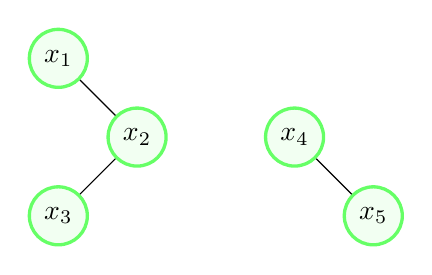
\begin{tikzpicture}[roundnode/.style={circle, draw=green!60, fill=green!5, very thick, minimum size=7mm}]
% Nodes
\node[roundnode] (x1) at (1, 2) {$x_1$};
\node[roundnode] (x2) at (2, 1) {$x_2$};
\node[roundnode] (x3) at (1, 0) {$x_3$};
\node[roundnode] (x4) at (4, 1) {$x_4$};
\node[roundnode] (x5) at (5, 0) {$x_5$};
\draw[] (x1) -- (x2);
\draw[] (x2) -- (x3);
\draw[] (x4) -- (x5);
\end{tikzpicture}
\caption{A simple graphical model with $p=5$ covariates.}
\label{fig:graphical_model}
\end{figure}



A special case is when the joint distribution is a multivariate Gaussian distribution, referred to as a Gaussian graphical model.  A Gaussian distribution is completely characterized by its mean $\mean \in \R^p$ and covariance matrix $\cov \in \R^{p\times p}$ and has the density
\begin{equation}
\phi(\bx) = \frac{1}{(2\pi)^{p/2} \sqrt{ |\det \cov| } } \exp \left( -\frac{1}{2}(\bx - \mean)^T \cov^{-1} (\bx - \mean)  \right)
\label{eq:gauss_density}
\end{equation}
whenever $\cov \succ 0$.  If $\cov$ has a zero eigenvalue, then the corresponding eigenvector indicates a direction in which the data does not vary.  We could alternatively specify the precision matrix $\preci = \cov^{-1}$, which is sometimes more useful.  The graph $\mathcal{G}$ has an intuitive structure given either the matrix $\cov$ or $\preci$.  If $\cov_{ij} = 0$, then $x_i$ and $x_j$ are independent, meaning they are a part of separate components.   If $\preci_{ij} = 0$, then $x_i$ and $x_j$ are conditionally independent given the remaining variables, meaning that there is no edge between the nodes corresponding to variables $x_i$ and $x_j$ (see \cite{GLASSO}).  For the example in figure~\ref{fig:graphical_model} the precision and covariance matrices would have the forms
\[
\cov = \begin{bmatrix}
* & * & * & 0 & 0\\
* & * & * & 0 & 0\\
* & * & * & 0 & 0\\
0 & 0 & 0 & * & *\\
0 & 0 & 0 & * & *\\
\end{bmatrix}, \quad 
\preci = \begin{bmatrix}
* & * & 0 & 0 & 0\\
* & * & * & 0 & 0\\
0 & * & * & 0 & 0\\
0 & 0 & 0 & * & *\\
0 & 0 & 0 & * & *\\
\end{bmatrix}
\]
where $*$ represents a non-zero element.  The block structure comes from the fact that there are two independent components in the graph.  To learn a Gaussian graphical model we just need to estimate the mean and covariance.



\subsection{Covariance estimation}

Given a random sample of data $\{ \bx_i \}_{i=1}^n \iid N(\mean, \cov)$, we can estimate the mean and covariance using maximum likelihood estimation.  The maximum likelihood estimate of $\mean$ is the sample mean $\bar{\bx} = \frac{1}{n}\sum_{i=1}^n \bx_i$ regardless of what $\cov$ is.  The likelihood function to be maximized is
\[
\underset{\cov \succeq 0}{\mathrm{maximize}}\  L(\cov) = \prod_{i=1}^n \frac{1}{(2\pi)^{p/2} \sqrt{|\det \cov| }} \exp\left( -\frac{1}{2}(\bx_i - \bar{\bx})^T \cov^{-1}(\bx_i - \bar{\bx})  \right)
\]
This is equivalent to minimizing the negative log-likelihood,
\[
\underset{\cov \succeq 0}{\mathrm{minimize}}\  - \log L(\cov) = \frac{np}{2} \log(2\pi) + \frac{n}{2} \log \det \cov - \frac{1}{2} \sum_{i=1}^n (\bx_i - \bar{\bx})^T \cov^{-1}(\bx_i - \bar{\bx})
\]
We can ignore the constants and it will also help to replace $\cov$ with $\preci^{-1}$ to avoid the inverse.
\[
\underset{\preci \succeq 0}{\mathrm{minimize}}\quad   -\log \det \preci +  \frac{1}{n}\sum_{i=1}^n (\bx_i - \bar{\bx})^T \preci (\bx_i - \bar{\bx})
\]
Since the sum is a scalar,
\[
\frac{1}{n}\sum_{i=1}^n (\bx_i - \bar{\bx})^T \preci (\bx_i - \bar{\bx}) = \tr{\frac{1}{n}\sum_{i=1}^n (\bx_i - \bar{\bx})^T \preci (\bx_i - \bar{\bx})} = \frac{1}{n}\sum_{i=1}^n \tr{  (\bx_i - \bar{\bx})^T \preci (\bx_i - \bar{\bx})}
\]
Using the trick that $\tr{AB} = \tr{BA}$, we simplify
\[
\frac{1}{n}\sum_{i=1}^n \tr{  (\bx_i - \bar{\bx})^T \preci (\bx_i - \bar{\bx})} = \frac{1}{n}\sum_{i=1}^n \tr{  (\bx_i - \bar{\bx})(\bx_i - \bar{\bx})^T \preci } = \tr{\frac{1}{n}\sum_{i=1}^n (\bx_i - \bar{\bx})(\bx_i - \bar{\bx})^T \preci  }
\]
However, the sample covariance matrix $\sampcov$ is given by
\[
\sampcov =  \frac{1}{n}\sum_{i=1}^n (\bx_i - \bar{\bx})(\bx_i - \bar{\bx})^T
\]
which means that the maximum likelihood problem becomes equivalent to
\begin{equation}
\underset{\preci \succeq 0}{\mathrm{minimize}}\quad   -\log \det \preci + \tr{\sampcov \preci}
\label{eq:cov_mle}
\end{equation}
This is a convex objective function (see \cite{BV}), but it is only defined whenever $\preci \succ 0$.  As long as this is the case, the objective is actually differentiable and the KKT conditions for the optimal solution are $-\preci^{-1} + \sampcov^T = 0$ (see \cite{matrixcookbook} for many useful matrix formulas).  Since $\sampcov$ is symmetric, we have the solution $\preci^{-1} = \cov = \sampcov$.  Of course, this is problematic if $\sampcov$ is not strictly positive definite.  In particular, this will always happen whenever there are more variables than samples, $p > n$, meaning that maximum likelihood estimation is ill-suited for high-dimensional problems.



\subsection{Sparsity and the graphical lasso}

The covariance, and equivalently the precision, matrix has $\frac{p(p+1)}{2}$ total entries that need to be estimated since it is symmetric.  In the high-dimensional setting when $p \gg n$, this is a huge number of parameters to estimate and we cannot hope to accurately estimate all of these given only a relatively small amount of data.  Instead we will try to only estimate a few important entries for $\preci$.  Similar to the lasso we will look for a sparse solution to the maximum likelihood problem, which is enforced by adding an $\ell_1$ regularizer to the objective function.
\begin{equation}
\underset{\preci \succeq 0}{\mathrm{minimize}}\  f(\preci) = - \log \det \preci + \tr{\sampcov \preci} + \lambda \|\preci\|_1
\label{eq:glasso_primal}
\end{equation}
We call the solution to this regularized problem the graphical lasso.  Here $\lambda > 0$ is the regularization parameter and the norm $\|\cdot \|_1$ is defined differently than the usual matrix 1-norm:
\[
\|\preci \|_1 = \sum_{i=1}^p \sum_{j=1}^p |\preci_{ij}|
\]
This is the same as the $\ell_1$ norm of the vectorized matrix $\mathrm{vec}\left( \preci \right)$.  Adding $\lambda \|\preci\|_1$ means that the objective function will remain convex, so this is still a semidefinite program (SDP) for the variable $\preci$.  Also note that since the only constraint on $\preci$ is that it is positive definite, Slater's condition holds and we have strong duality.\\

To derive the dual SDP we need to use the fact that the vector $\ell_1$ and $\ell_{\infty}$ norms are dual.  We use the notation $\|\cdot\|_{\infty}$ to refer to the $\ell_{\infty}$ norm of the vectorized matrix, not to the usual matrix $\infty$-norm.
\[
\| \dualvar \|_{\infty} = \max_{i,j=1,\ldots,p} \left| \dualvar_{ij} \right|
\]
Therefore, we can write
\[
\underset{\preci \succeq 0}{\min}\  - \log \det \preci + \tr{\sampcov \preci} + \lambda \|\preci\|_1 
= \underset{\preci \succeq 0}{\min}\  - \log \det \preci + \tr{\sampcov \preci} + \lambda\  \underset{\|  \dualvar \|_{\infty} \le 1}{\max}\ \tr{ \preci \dualvar }
\]
Of course we can rescale $\dualvar$ to obtain the equivalent min-max problem
\[
\underset{\preci \succeq 0}{\min}\  \underset{\|  \dualvar \|_{\infty} \le \lambda }{\max}\  - \log \det \preci + \  \tr{ \preci \left(\sampcov + \dualvar \right) }
\]
By strong duality, this is equivalent to
\[
 \underset{\|  \dualvar \|_{\infty} \le \lambda }{\max}\ \underset{\preci \succeq 0}{\min}\  - \log \det \preci + \  \tr{ \preci \left(\sampcov + \dualvar \right) }
\] 
We have already solved this minimization problem in \ref{eq:cov_mle}, although with $\sampcov + \dualvar$ replaced with $\sampcov$ and the optimal solution is $\preci = \left(  \sampcov + \dualvar \right)^{-1}$.  Plugging this in gives
\[
\log \det  \left(  \sampcov + \dualvar \right)  + \  \tr{ \eye } = \log \det  \left(  \sampcov + \dualvar \right)  + p
\]
meaning that the dual SDP of \ref{eq:glasso_primal} is
\begin{align}
\begin{split}
\underset{\dualvar \succeq 0}{\mathrm{maximize}}\ &g(\dualvar) =  \log \det\left( \sampcov + \dualvar \right) + p\\
\text{subject to}\quad  &\| \dualvar \|_{\infty} \le \lambda
\end{split}
\label{eq:glasso_dual}
\end{align}
where the dual variable satisfies $\dualvar + \sampcov = \preci^{-1} = \cov$.  The box constraint on the dual variable says that the estimated covariance matrix cannot be further than $\lambda$ from the sample covariance $\sampcov$ in this norm.\\



Since strong duality holds for the graphical lasso problem we can equivalently solve either the primal or dual SDP.  For the primal SDP the variable is the precision matrix, whereas the variable in the dual SDP is $\dualvar = \cov - \sampcov$, meaning the variable is essentially the covariance matrix.  In terms of our graphical model $\mathcal{G}$, a sparse precision matrix means that most pairs of variables $x_i,x_j$ will be conditionally independent of each other given the remaining variables.  That is, these nodes are not direct neighbors.  A sparse precision matrix does not imply that the covariance is sparse, however, so the variables may all still be dependent on each other.  A sparse precision matrix just means that the graph $\mathcal{G}$ does not have many large cliques.  A practical benefit of using a sparse estimate of the precision matrix is that the model is more readily interpretable with clear dependencies between variables.  In the next section we consider several algorithms that solve either the primal SDP \ref{eq:glasso_primal} or the dual SDP \ref{eq:glasso_dual}.



\section{Computing the graphical lasso solution}

Since \ref{eq:glasso_primal} and \ref{eq:glasso_dual} are SDPs we can solve them using CVX in Matlab, which will then use the SDPT3 solver.  We quickly find that this method becomes extremely slow once the dimension $p$ is around 50.  For large graphical models, this is insufficient and so we will now look at several algorithms designed specifically for the graphical lasso problem.  For most of these algorithms the basic building block is coordinate descent.

\subsection{Coordinate descent algorithms}

Coordinate descent (CD) algorithms are extremely simple algorithms that minimize only along one coordinate at a time as opposed to methods like gradient descent, which updates all coordinates after every iteration.

\begin{algorithm}
\SetAlgoLined
\KwIn{ Objective function $f$, starting point $\bx_0 \in \R^d$}
\KwResult{Optimal solution $\bx^*$ and value $f(\bx^*)$}
Initialize $k=0$, $\bx^{(k)} = \bx_0$\;
\While{not converged}{
$i \leftarrow \mod(k,d) + 1$\;
$x^{(k+1)}_i \leftarrow \underset{x\in \R}{\mathrm{argmin}}\ f(x^{k}_1,\ldots,x^{(k)}_{i-1},x, x^{(k)}_{i+1}\ldots,x^{(k)}_d)  $\;
$k \leftarrow k + 1$\;
}
\caption{Coordinate descent algorithm}
\label{alg:cd}
\end{algorithm}

Algorithm~\ref{alg:cd} shows the basic coordinate descent algorithm where exact minimization is done along each coordinate.  This is not always possible and in these cases one can use gradient descent with line search.  For simple quadratic problems, though, we can find the exact minimizer at each step.  Under some technical assumptions including strong convexity, continuously differentiable, and Lipschitz it can be shown (see Theorem 3 and Assumption 1 of \cite{CD}) that coordinate descent converges linearly.
\begin{equation}
f(\bx^{(k)}) - f(\bx^*) \le \left( 1 - c \right)^{k/d} \left( f(\bx_0) - f(\bx^*) \right)
\label{eq:cd_linear}
\end{equation}
for $k=nd$ with $n = 1,2,3,\ldots$ and where the constant $c > 0$ depends proportionally on the strong convexity constant and inverse proportionally on the dimension $d$ and Lipschitz constant.  This is a result on the objective function after every complete cycle through all coordinates, where $\lfloor k/d \rfloor$ is the number of total cycles that have been completed by iteration $k$.  For the convergence criteria we can set a tolerance $\epsilon$ on either the relative change in the objective function value
\[
\frac{f(\bx^{((n-1)d)}) - f(\bx^{(nd)}) }{| f(\bx^{((n-1)d)}) | } < \epsilon
\]
or the relative change in the solution
\[
\frac{\| \bx^{(nd)} - \bx^{((n-1)d)} \| }{ \| \bx^{((n-1)d)} \|} < \epsilon
\]
where $k = nd$ for $n=1,2,3,\ldots$ meaning we only check the convergence criteria after each complete cycle over all of the coordinates.\\

Two important problems that can be solved with coordinate descent and are useful for the algorithms presented in the next section are the lasso problem:
\begin{equation}
\underset{ \bx \in \R^d }{\mathrm{minimize}}\ \frac{1}{2} \bx^T {\boldsymbol A} \bx + {\boldsymbol b}^T \bx + \lambda \|\bx\|_1
\label{eq:lasso}
\end{equation}
and a quadratic program (QP) with box constraints:
\begin{align}
\begin{split}
\underset{ \bx \in \R^d }{\mathrm{minimize}}\quad &\frac{1}{2}\bx^T {\boldsymbol A} \bx + {\boldsymbol b}^T \bx \\
\text{subject to}\quad& {\boldsymbol \ell} \le \bx \le {\boldsymbol u}
\end{split}
\label{eq:box_qp}
\end{align}
Note that equation~\ref{eq:lasso} is written differently from how the lasso problem is usually defined.  In both problems, ${\boldsymbol A}$ is a symmetric positive semidefinite matrix.\\

For the lasso problem, the optimality condition for the update to variable $x_i$ can be found by setting the subgradient of the function $x\mapsto f(x_1,\ldots,x_{i-1}, x , x_{i+1}, \ldots, x_d)$ to zero.
\[
A_{ii}x_i + \sum_{j\neq i}A_{ij}x_j + b_i + \lambda \gamma_i = 0
\] 
where the subgradient $\gamma_i \in \partial |x|$
\[
\gamma_i \in  \begin{cases}
\{-1\}  & x_i < 0\\
\{1\}   & x_i > 0\\
[-1,1] & x_i = 0
\end{cases}
\]
In vector form this is 
\begin{equation}
{\boldsymbol A}\bx + {\boldsymbol b} + \lambda {\boldsymbol \gamma} = \bzero
\label{eq:lasso_kkt}
\end{equation}
Since ${\boldsymbol A} \succ 0$ we know that $A_{ii} > 0$ and $\sgn{x_i} = \sgn{A_{ii}x_i}$.  Now consider three cases.  If $x_i > 0$, then $\gamma_i = 1$ and
\[
A_{ii}x_i = - \sum_{j\neq i}A_{ij}x_j - b_i - \lambda
\]
Since $\lambda > 0$ we know that $- \sum_{j\neq i}A_{ij}x_j - b_i > 0$ as well so we can write
\[
x_i = \frac{ \left| - \sum_{j\neq i}A_{ij}x_j - b_i \right| - \lambda }{A_{ii}}
\]
assuming $x_i > 0$.  For $x_i < 0$ we can follow similar steps with $\gamma_i = -1$ now.
\[
x_i = \frac{- \sum_{j\neq i}A_{ij}x_j - b_i + \lambda}{A_{ii}} = -\left( \frac{\left| - \sum_{j\neq i}A_{ij}x_j - b_i \right| - \lambda}{A_{ii}} \right)
\]
since $- \sum_{j\neq i}A_{ij}x_j - b_i < 0$ in this case.
In the last case we just have $x_i=0$.  We can now write the formula for the update to the variable $x_i$
\begin{equation}
x_i \leftarrow \sgn{  - \sum_{j\neq i}A_{ij}x_j - b_i  } \left(  \frac{\left| - \sum_{j\neq i}A_{ij}x_j - b_i \right| - \lambda}{A_{ii}} \right)^+
\label{eq:lasso_update}
\end{equation}
with $z^+ = \max\{0,z\}$.  This is just soft thresholding and we use this update formula in algorithm~\ref{alg:cd} to solve the lasso problem~\ref{eq:lasso}.\\


For the quadratic program with box constraints the update is even simpler since the objective function is quadratic.  Specifically, $x\mapsto f(x_1,\ldots,x_{i-1}, x , x_{i+1}, \ldots, x_d)$ is a quadratic function with positive leading coefficient since ${\boldsymbol A} \succ 0$.  Setting the derivative to zero gives
\[
x^* =  \frac{-\sum_{j\neq i} A_{ij}x_j  - b_i}{ A_{ii} }
\]
as the optimal point.  However, we have to enforce the constraint that $\ell_i \le x_i \le u_i$.  Because the leading coefficient is positive, the function is decreasing on $(-\infty, x^*]$ and increasing on $[x^*,\infty)$.  Therefore, the update is given by taking $x_i$ to be the point in the box $[\ell_i, u_i]$ that is as close to $x^*$ as possible
\begin{equation}
x_i \leftarrow  \begin{cases}
\ell_i & x^* \le \ell_i\\
x^* & \ell_i \le x_i \le u_i\\
u_i & x^* \ge u_i
\end{cases}, \quad \text{ with } \quad 
x^* =  \frac{-\sum_{j\neq i} A_{ij}x_j  - b_i}{ A_{ii} }
\label{eq:boxqp_update}
\end{equation}
Using this update formula in algorithm~\ref{alg:cd} will solve the quadratic program with box constraints~\ref{eq:box_qp}.\\


%By a change of variables $\bx = \bg + \frac{{\boldsymbol u} + {\boldsymbol \ell}}{2}$, \ref{eq:box_qp} is equivalent to the symmetric problem
%\begin{align}
%\begin{split}
%\underset{ \bg \in \R^d }{\mathrm{minimize}}\quad &\frac{1}{2}\left( \bg + \frac{{\boldsymbol u} + {\boldsymbol \ell}}{2} \right)^T {\boldsymbol A} \left( \bg + \frac{{\boldsymbol u} + {\boldsymbol \ell}}{2} \right)+ {\boldsymbol b}^T  \left( \bg + \frac{{\boldsymbol u} + {\boldsymbol \ell}}{2} \right) \\
%\text{subject to}\quad&  |\bg| \ \le \frac{{\boldsymbol u} - {\boldsymbol \ell}}{2}
%\end{split}
%\label{eq:box_qp2}
%\end{align}
%with $\bg = \bzero$ corresponding to the center of the box.  This form will be especially useful later on.\\


These special cases are implemented in the Matlab functions \texttt{lasso.m} and \texttt{QP\_box.m}, respectively \footnote{See the end of this report for the code listings.}.  The implementations were verified against CVX for relatively small random problems of dimension around $d=20$.  Figure~\ref{fig:CD_convergence} shows that for both problems we have the theoretical linear convergence given by equation~\ref{eq:cd_linear}.  We also see from comparing the top and bottom rows that increasing the eigenvalues of ${\boldsymbol A}$ makes the problem more convex and we require fewer iterations in both algorithms.  For the lasso problem, increasing $\lambda$ has a similar effect in that fewer iterations are needed for convergence, but also that the computed solution is more sparse.  Of course, neither of these two algorithms can be used directly to solve the original problem \ref{eq:glasso_primal} that we are interested in, but they can be used as building blocks to compute the solution one row and column at a time.
 

\begin{figure}
\centering
\includegraphics[width=\textwidth]{plots/CD_convergence.png}
\caption{Performance of the CD algorithm~\ref{alg:cd} on the QP with box constraints~\ref{eq:box_qp} (left column in blue) and the lasso problem~\ref{eq:lasso} (right column in red) on random problems of dimension $d=50$.  In all cases we set a tolerance of $\epsilon = 10^{-12}$ on the relative difference of objective function values and for the lasso problem we set $\lambda = 1$.  The top row shows the performance on a random problem where ${\boldsymbol A} = {\boldsymbol B}^T {\boldsymbol B} + {\boldsymbol I}$, where ${\boldsymbol B} \in \R^{d\times d}$ is a random matrix and ${\boldsymbol I}$ is the identity, ensuring that the smallest eigenvalue of ${\boldsymbol A}$ is at least 1.  For the bottom row we use ${\boldsymbol A} = {\boldsymbol B}^T {\boldsymbol B} + 10\times {\boldsymbol I}$, so that the smallest eigenvalues is now at least 10.}
\label{fig:CD_convergence}
\end{figure}






\subsection{Glasso and DP-Glasso}

The most common approaches to solving either \ref{eq:glasso_primal} or \ref{eq:glasso_dual} revolve around partitioning the covariance and precision matrices and updating them one row and column at a time in a coordinate descent-like fashion (see \cite{GLASSO}, \cite{Banerjee}, and \cite{MH}).  We will use notation consistent with these papers.  Let $\preci_{-i,-i}$ denote the $(p-1) \times (p-1)$ submatrix obtained by deleting the $i$-th row and column from $\preci$, let $\spreci_{-i,i}$ be the $(p-1) \times 1$ column vector obtained by deleting the $i$-th entry from the $i$-th column of $\preci$, and let $\sspreci_{i,i} = \preci_{i,i}$.  If we rearrange the rows and columns of $\preci$ so that the $i$-th row and column is now last, then we can write
\[
\preci  = \begin{bmatrix}
\preci_{-i,-i} & \spreci_{-i,i}\\
\spreci_{-i,i}^T & \sspreci_{i,i}
\end{bmatrix}
= \begin{bmatrix}
\preci_{11} & \spreci_{12}\\
\spreci_{12}^T & \sspreci_{22}
\end{bmatrix}
\]
We will use the simpler notation on the right with $\preci_{11}, \spreci_{12}, \sspreci_{22}$ where the coordinate is now implicit and will be clear from context.  We define $\cov_{11},\scov_{12},\sscov_{22}$ similarly for the covariance matrix as well as $\ssampcov_{12}$ for the sample covariance matrix.  Any other block matrices in the following will also use this notation.  The relation between the blocks of $\preci$ and $\cov$ is given by the Schur complement since $\preci^{-1} = \cov$.
\begin{equation}
\begin{bmatrix}
\cov_{11} & \scov_{12}\\
\scov_{12}^T & \sscov_{22}
\end{bmatrix}
= \begin{bmatrix}
\preci_{11}^{-1} + \frac{\preci_{11}^{-1} \spreci_{12} \spreci_{12}^T \preci_{11}^{-1} }{\sspreci_{22} - \spreci_{12}^T \preci_{11}^{-1} \spreci_{12} } 
& -\frac{  \preci_{11}^{-1} \spreci_{12} }{ \sspreci_{22} - \spreci_{12}^T \preci_{11}^{-1} \spreci_{12} }\\[8pt]
-\frac{  \spreci_{12}^T \preci_{11}^{-1}  }{ \sspreci_{22} - \spreci_{12}^T \preci_{11}^{-1} \spreci_{12} }
& \frac{  1 }{ \sspreci_{22} - \spreci_{12}^T \preci_{11}^{-1} \spreci_{12} }
\end{bmatrix}
\label{eq:schur}
\end{equation}
We can derive another useful relation by using the fact that $\preci \cov = \eye$, which gives a system of four equations:
\begin{align*}
\cov_{11}\preci_{11} + \scov_{12} \spreci_{21} &= \eye\\
\scov_{21} \preci_{11} + \sscov_{22}\spreci_{21} &= \bzero\\
\cov_{11}\spreci_{12} + \scov_{12}\sspreci_{22} &= \bzero\\
\scov_{21} \spreci_{12} + \sscov_{22} \sspreci_{22} &= 1
\end{align*}
By rearranging these equations we obtain the relation\footnote{The bottom-right entry is actually slightly wrong in the paper \cite{MH}, although this particular relation is not used anywhere else.}
\begin{equation}
\begin{bmatrix}
\cov_{11} & \scov_{12}\\
\scov_{12}^T & \sscov_{22}
\end{bmatrix}
= \begin{bmatrix}
\left( \preci_{11} - \frac{\spreci_{12}\spreci_{21}}{\sspreci_{22}} \right)^{-1} 
& -\cov_{11} \frac{\spreci_{12}}{\sspreci_{22}} \\[8pt]
-\cov_{11} \frac{\spreci_{12}}{\sspreci_{22}}
& \frac{1}{\sspreci_{22}}\left( 1 + \frac{ \spreci_{21} \cov_{11} \spreci_{12} }{\sspreci_{22}}  \right)
\end{bmatrix}
\label{eq:schur2}
\end{equation}
The relations \ref{eq:schur} and \ref{eq:schur2} will be essential for switching between $\cov$ and $\preci$ whenever the rows and columns are updated.



\subsubsection{Glasso}

The first of these types of algorithms is the original Glasso algorithm introduced in \cite{GLASSO} and largely based on the work done in \cite{Banerjee}.  As a starting point consider the optimality conditions for \ref{eq:glasso_primal} and finding a zero subgradient.  The matrix derivative of the objective function is
\begin{equation}
-\preci^{-1} + \sampcov + \lambda \bsgn = \bzero
\label{eq:primal_kkt}
\end{equation}
where each entry $\gamma_{ij} = \bsgn_{ij}$ is in the subdifferential $\partial |x|$ at $x = \preci_{ij}$ just as in the lasso problem \ref{eq:lasso}.  Instead of trying to solve for $\preci$ the Glasso algorithm solves for $\cov$ which satisfies
\[
\cov - \sampcov - \lambda \bsgn = \bzero
\]
By looking at the upper-right block and using equation~\ref{eq:schur2} for $\scov_{12}$ we obtain
\[
\cov_{11} \frac{\spreci_{12}}{\sspreci_{22}} + \ssampcov_{12} + \lambda \bsgn_{12} = \bzero
\]
Because $\preci \succ 0$, $\sspreci_{22} > 0$ and $\sgn{\spreci_{12}/\sspreci_{22}} = \bsgn_{12}$, so this is exactly the optimality condition we derived for the lasso problem \ref{eq:lasso} whenever ${\boldsymbol A}= \cov_{11}$, ${\boldsymbol b} = \ssampcov_{12}$ and ${\boldsymbol \gamma} = \bsgn_{12}$.  The solution of this lasso problem is $\spreci_{12}/\sspreci_{22}$, which we can then use to update $\scov_{12}$ and build an estimate of the inverse $\preci$ using equations~\ref{eq:schur} and \ref{eq:schur2}.  We repeat this procedure, cycling over all of the rows and columns of $\cov$ until convergence.  Algorithm~\ref{alg:glasso} describes the procedure, which is implemented in the Matlab function \texttt{glasso.m}.\\

\begin{algorithm}
\SetAlgoLined
\KwIn{Sample covariance $\sampcov$, regularization parameter $\lambda$}
\KwResult{Estimated precision $\preci$ and covariance $\cov$}
Initialize $\cov = \sampcov + \lambda \eye$, $\preci = \eye$, $k = 0$\;
\While{not converged}{
$i \leftarrow \mod(k,p) + 1$\; 
$\bx \leftarrow  \texttt{lasso}(\cov_{11}, \ssampcov_{12}, \lambda)$ \tcp*{$\bx = \spreci_{12}/\sspreci_{22}$}\
$\scov_{12} \leftarrow -\cov_{11}\bx$ \tcp*{update covariance}
$\sspreci_{22} \leftarrow 1/(\sscov_{22} + \bx^T \scov_{12})$ \tcp*{update precision}
$\spreci_{12} \leftarrow \sspreci_{22}\bx$\;
$k\leftarrow k + 1$\;
}
\caption{Glasso}
\label{alg:glasso}
\end{algorithm}

If $\lambda$ is large, then the solution $\bx$ returned by \texttt{lasso} should be sparse, which means that we are updating the rows and columns of the matrix $\preci$ with sparse vectors resulting in a sparse matrix.\\

There are several problems with the Glasso algorithm, which are discussed in detail in \cite{MH}.  Perhaps the biggest is that the primal objective function \ref{eq:glasso_primal} may not decrease monotonically.  Note that the matrix $\cov_{11}$ and variable $\spreci_{12}$ in the lasso problem are actually coupled.  This means after that each iteration we may not have $\preci^{-1} = \cov$, so the dual variable $\dualvar \neq \cov - \sampcov$.  However, it turns out that algorithm~\ref{alg:glasso} actually does coordinate ascent on the dual problem \ref{eq:glasso_dual} (Theorem 4.1 of \cite{MH}).  This is illustrated in figure~\ref{fig:glasso_primaldual} where the dual objective is seen to be monotonically increasing.  Using the starting point $\cov = \sampcov + \lambda \eye$ ensures that $\cov$ is dual feasible and positive definite.  This will ensure that $\cov$ remains positive definite throughout.  However, because $\preci \neq \cov^{-1}$ we are not guaranteed that $\preci$ is also positive definite at any given step.  Despite this, once the algorithm converges all rows and columns of $\preci$ are updated and it will be the inverse $\cov^{-1}$.  Since our goal is to uncover the structure of the graphical model through $\preci$ it may be better to ensure that $\preci$ is always positive definite.  This is what the next algorithm DP-Glasso attempts to do.


\begin{figure}
\centering
\includegraphics[width=\textwidth]{plots/glasso_primaldual.png}
\caption{The primal (blue) and dual (red) objective values at each iteration of the Glasso algorithm on a random problem of dimension $p=50$.  Here $\sampcov$ is the sample covariance of $n=5$ data points drawn from a $N(\bzero, 1.2^2\times \eye)$ distribution and $\lambda = 0.5$.  The left plot shows the primal objective values $f(\preci)$ and the dual objective values $g(\cov)$ while the right plot shows the primal objective values $f(\cov^{-1})$ using the true primal variable as well as the dual objective values $g(\cov)$.  In the left plot the two curves cross indicating that $\preci$ is not primal feasible (i.e. not positive definite).}
\label{fig:glasso_primaldual}
\end{figure} 





\subsubsection{DP-Glasso}

In many ways the DP-Glasso algorithm is opposite to the Glasso algorithm.  The Glasso algorithm starts from the KKT optimality conditions~\ref{eq:primal_kkt} of the primal problem \ref{eq:glasso_primal} to derive a condition on the block $\scov_{12}$.  This condition is translated using~\ref{eq:schur} and~\ref{eq:schur2} to a condition on the primal variable $\spreci_{12}$ and is recognized to be the optimality conditions for the lasso problem~\ref{eq:lasso_kkt}, which is then solved to update $\preci$ and $\cov$.  The DP-Glasso does all of this except from the point of view of the dual problem.  Rather than go through the tedious derivations we refer the reader to \cite{MH} and instead present a diagram~\ref{fig:primaldual_diagram} that summarizes the relationship nicely.  The DP-Glasso algorithm itself is outlined in algorithm~\ref{alg:dpglasso} and implemented in the Matlab function \texttt{dpglasso.m}.\\

\begin{figure}
\centering
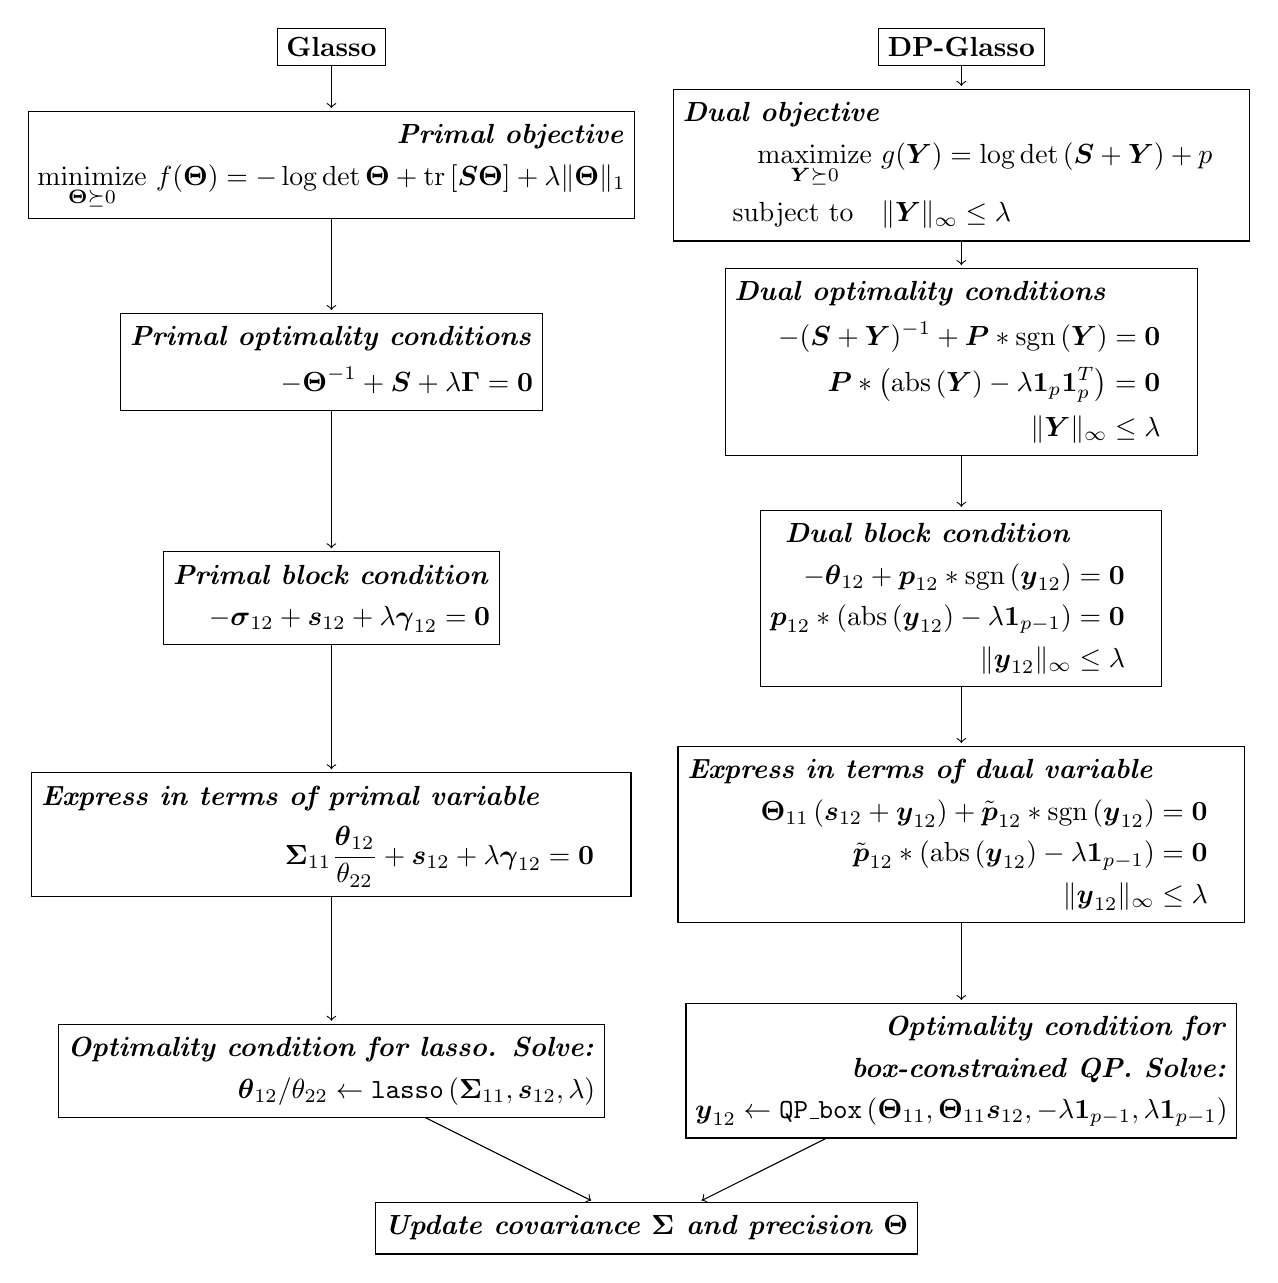
\begin{tikzpicture}[every node/.style={rectangle,draw}, shorten >=1pt,node distance=5cm,on grid,auto]
% Define all the nodes.
% Glasso 
\node (glasso) at (-4,0) {\bf Glasso};
% DP-Glasso
\node (dpglasso) at (4,0) {\bf DP-Glasso};
% Dual objective
\node (dual_obj) at (4,-1.5){
$\begin{aligned}
\text{\bf \emph{Dual objective}}\\
\underset{\dualvar \succeq 0}{\mathrm{maximize}}\ &g(\dualvar) =  \log \det\left( \sampcov + \dualvar \right) + p\\
\text{subject to}\quad  &\| \dualvar \|_{\infty} \le \lambda
\end{aligned}$
};
% Primal objective
\node (primal_obj) at (-4, -1.5) {
$\begin{aligned}
\text{\bf \emph{Primal objective}}\\
\underset{\preci \succeq 0}{\mathrm{minimize}}\  f(\preci) = - \log \det \preci + \tr{\sampcov \preci} + \lambda \|\preci\|_1
\end{aligned}$
};
% Dual KKT
\node (dual_kkt) at (4, -4) {
$\begin{aligned}
\text{\bf \emph{Dual optimality conditions}}\\
-(\sampcov + \dualvar)^{-1} + \bP* \sgn{\dualvar} &= \bzero\\
\bP*\left( \abs{\dualvar} - \lambda \one_p \one_p^T \right) &= \bzero\\
\|\dualvar\|_{\infty} &\le \lambda
\end{aligned}$
};
% Primal KKT
\node (primal_kkt) at (-4, -4) {
$\begin{aligned}
\text{\bf \emph{Primal optimality conditions}}\\
-\preci^{-1} + \sampcov + \lambda \bsgn = \bzero
\end{aligned}$
};
% Primal block condition
\node (primal_block) at (-4, -7) {
$\begin{aligned}
\text{\bf \emph{Primal block condition}}\\
-\scov_{12} + \ssampcov_{12} + \lambda \bg_{12} = \bzero
\end{aligned}$
};
% Dual block condition
\node (dual_block) at (4, -7.0) {
$\begin{aligned}
\text{\bf \emph{Dual block condition}}\\
-\spreci_{12} + \bp_{12}*\sgn{\by_{12}} &= \bzero\\
\bp_{12}*\left( \abs{\by_{12}} - \lambda \one_{p-1}\right) &= \bzero\\
\|\by_{12}\|_{\infty} &\le \lambda
\end{aligned}$
};
% Express primal
\node (express_primal) at (-4, -10) {
$\begin{aligned}
\text{\bf \emph{Express in terms of primal variable}}\\
\cov_{11} \frac{\spreci_{12}}{\sspreci_{22}} + \ssampcov_{12} + \lambda \bg_{12} &= \bzero
\end{aligned}$
};
% Express dual
\node (express_dual) at (4, -10) {
$\begin{aligned}
\text{\bf \emph{Express in terms of dual variable}}\\
\preci_{11}\left( \ssampcov_{12} + \by_{12} \right) + \tilde{\bp}_{12}*\sgn{ \by_{12} } &= \bzero\\
\tilde{\bp}_{12}*\left( \abs{\by_{12}} - \lambda \one_{p-1}\right) &= \bzero\\
\|\by_{12}\|_{\infty} &\le \lambda
\end{aligned}$
};
% Stationary lasso
\node (stat_lasso) at (-4, -13) {
$\begin{aligned}
\text{\bf \emph{Optimality condition for lasso.  Solve:}}\\
\spreci_{12}/\sspreci_{22} \leftarrow \texttt{lasso}\left( \cov_{11}, \ssampcov_{12}, \lambda \right)
\end{aligned}$
};
% Stationary QP box
\node (stat_qpbox) at (4, -13) {
$\begin{aligned}
\text{\bf \emph{Optimality condition for}}\\
\text{\bf \emph{box-constrained QP.  Solve:}}\\
 \by_{12} \leftarrow \texttt{QP\_box}\left( \preci_{11}, \preci_{11}\ssampcov_{12}, -\lambda\one_{p-1}, \lambda \one_{p-1}  \right)
\end{aligned}$
};
% Update
\node (update) at (0, -15) {
$\begin{aligned}
\text{\bf \emph{Update covariance $\cov$ and precision $\preci$}}\\
\end{aligned}$
};
% Draw the arrows
\draw[->] (glasso) -- (primal_obj);
\draw[->] (dpglasso) -- (dual_obj);
\draw[->] (primal_obj) -- (primal_kkt);
\draw[->] (dual_obj) -- (dual_kkt);
\draw[->] (primal_kkt) -- (primal_block);
\draw[->] (dual_kkt) -- (dual_block);
\draw[->] (primal_block) -- (express_primal);
\draw[->] (dual_block) -- (express_dual);
\draw[->] (express_primal) -- (stat_lasso);
\draw[->] (express_dual) -- (stat_qpbox);
\draw[->] (stat_lasso) -- (update);
\draw[->] (stat_qpbox) -- (update);
\end{tikzpicture}
\caption{A summary of the derivations of the Glasso and DP-Glasso algorithms presented in \cite{MH} and \cite{GLASSO}.  The matrix $\bP = \abs{\preci}$ has non-negative entries, $\tilde{\bp}_{12} = \bp_{12}/\sscov_{22}$ (recall $\sscov_{22} = s_{22} + \lambda$), and $\one_p$ is a $p\times 1$ vector of all 1's.}
\label{fig:primaldual_diagram}
\end{figure}



%Recall that the problematic line in the Glasso algorithm was computing the solution to
%\[
%\cov_{11} \frac{\spreci_{12}}{\sspreci_{22}} + \ssampcov_{12} + \lambda \bsgn_{12} = \bzero
%\]
%using $\texttt{lasso}(\cov_{11}, \ssampcov_{12}, \lambda)$ since $\cov_{11}$ depends on $\spreci_{12}$.  We can instead use the relationships in~\ref{eq:schur} to see that
%\[
%\sscov_{22}\preci_{11}^{-1} \spreci_{12} + \ssampcov_{12} + \lambda \bsgn_{12} = \bzero
%\]
%so that $\preci_{11}^{-1}$ and $\spreci_{12}$ do not depend on each other.  From the original equation~\ref{eq:primal_kkt} we know that $\sscov_{22} > 0$ since $\cov \succ 0$ and therefore, $\gamma_{22} = 1$ for the subgradient.  Hence $\sscov_{22} = s_{22} + \lambda$ is actually fixed.  In fact, the authors of \cite{MH} propose another algorithm called P-Glasso, which uses this equation as well as equations~\ref{eq:schur} and \ref{eq:schur2} to correct $\preci$ at each iteration so $\preci^{-1} = \cov$.  However, each correction is a rank-one update requiring $O(p^2)$ operations, which can quickly add up.  Instead DP-Glasso






\begin{algorithm}
\SetAlgoLined
\KwIn{Sample covariance $\sampcov$, regularization parameter $\lambda$}
\KwResult{Estimated precision $\preci$ and covariance $\cov$}
Initialize $\cov = \sampcov + \lambda \eye$, $\preci = \eye$, $k = 0$\;
\While{not converged}{
$i \leftarrow \mod(k,p) + 1$\; 
$\by \leftarrow  \texttt{QP\_box}(\preci_{11}, \preci_{11}\ssampcov_{12}, -\lambda \one_{p-1}, \lambda \one_{p-1})$ \tcp*{$\scov_{12} = \by_{12} + \ssampcov_{12}$}\
$\scov_{12} \leftarrow \by_{12} + \ssampcov_{12}$ \tcp*{update covariance}
$\spreci_{12} \leftarrow -\preci_{11}\scov_{12}/\sscov_{22}$  \tcp*{update precision}
$\sspreci_{22} \leftarrow  (1 - \spreci_{12}^T\scov_{12} )/\sscov_{22} $\;
$k\leftarrow k + 1$\;
}
\caption{DP-Glasso}
\label{alg:dpglasso}
\end{algorithm}


Based on figure~\ref{fig:primaldual_diagram} we expect that DP-Glasso will have the same problem that Glasso has only for the covariance matrix $\cov$.  Figure~\ref{fig:dpglasso_primaldual} shows that this is indeed the case where the dual objective is now the one that is not monotone increasing.  This is to be expected because the box-constrained QP that solves for $\by_{12}$ depends on $\preci_{11}$, which is coupled with $\by_{12}$.  In fact the authors of \cite{MH} propose a corrected version called P-Glasso, which uses equation~\ref{eq:schur} to enforce that $\preci = \cov^{-1}$ after each iteration in Glasso.  In the diagram~\ref{fig:primaldual_diagram} this corresponds to changing the expression in terms of the primal variable.  The same could in theory be done for DP-Glasso.  Each correction however is a rank one update and costs $O(p^2)$ operations.  Since Glasso returns $\cov$ and DP-Glasso returns $\preci$ there is really no need to use P-Glasso unless one needs both matrices at once.  Moreover, upon convergence we have that $\preci^{-1} = \cov$ for both Glasso and DP-Glasso (P-Glasso guarantees this pre-asymptotically).


\begin{figure}
\centering
\includegraphics[width=\textwidth]{plots/dpglasso_primaldual.png}
\caption{The primal (blue) and dual (red) objective values at each iteration of the DP-Glasso algorithm on a random problem of dimension $p=50$.  Here $\sampcov$ is the sample covariance of $n=5$ data points drawn from a $N(\bzero, 16\times \eye)$ distribution and $\lambda = 0.5$.  The left plot shows the primal objective values $f(\preci)$ and the dual objective values $g(\cov)$ while the right plot shows the primal objective values $f(\preci)$ and the dual objective values $g(\preci^{-1}-\sampcov)$ using the true dual variable.}
\label{fig:dpglasso_primaldual}
\end{figure}







\subsection{ADMM}

A completely different approach for solving the primal problem \ref{eq:glasso_primal}, which is not based on coordinate descent, is the alternating direction method of multipliers (ADMM) (see \cite{ADMM} and \cite{princetonlecture}).  The problem is equivalent to
\begin{align*}
\underset{\preci \succeq 0}{\mathrm{minimize}}&\quad - \log \det \preci + \tr{\sampcov \preci} + \lambda \| \bZ\|_1\\
\text{subject to}&\quad \preci = \bZ
\end{align*}
If $\mu$ is the penalty parameter, then the augmented Lagrangian is
\[
L(\preci, \bZ, \dualvar) = - \log \det \preci + \tr{\sampcov \preci} + \lambda \| \bZ\|_1 + \tr{\dualvar\left( \preci - \bZ \right)} + \frac{\mu}{2}\|\preci - \bZ\|_{F}^2
\]
Note that the dual variable $\dualvar$ is exactly the dual variable we have seen before, $\dualvar + \sampcov = \preci^{-1}$, meaning at the end of the algorithm we will easily be able to recover the exact inverse $\cov$.  ADMM alternates between minimizing over $\preci$ and $\bZ$.  At iteration $k$ the minimization over $\preci$ is given by
\[
\preci^{(k+1)} = \underset{\preci \succeq 0}{\mathrm{argmin}}\   L(\preci, \bZ^{(k)}, \dualvar^{(k)}) 
\]
Now the objective is differentiable with respect to $\preci$ so setting the matrix derivative to zero gives the optimality condition
\[
\preci - \frac{1}{\mu}\preci^{-1} = \bZ^{(k)} - \frac{1}{\mu} \sampcov - \frac{1}{\mu}\dualvar^{(k)}
\]
Therefore, the eigenvalues of the matrix on the left and right must agree (see \cite{princetonlecture}).  Let the eigendecomposition of the right-hand side (which is a symmetric matrix) be
\[
{\boldsymbol V}{\boldsymbol \Lambda}{\boldsymbol V}^T = \bZ^{(k)} - \frac{1}{\mu} \sampcov - \frac{1}{\mu}\dualvar^{(k)} = \preci - \frac{1}{\mu}\preci^{-1}
\]
The eigenvalues $\rho_i$ of $\preci$ must satisfy
\[
\rho_i - \frac{1}{\rho_i \mu} = \lambda_i
\]
where $\lambda_i$ is an eigenvalue on the diagonal of ${\boldsymbol \Lambda}$.  Solving the quadratic equation and using the fact that $\rho_i > 0$ gives
\[
\preci^{(k+1)} = \frac{1}{2} {\boldsymbol V} \diag{ \lambda_i  + \sqrt{\lambda_i^2 + \frac{4}{\mu}} } {\boldsymbol V}^T
\]
The next step in ADMM is minimization over $\bZ$:
\[
\bZ^{(k+1)} = \underset{\bZ \succeq 0}{\mathrm{argmin}}\   L(\preci^{(k+1)}, \bZ, \dualvar^{(k)}) 
\]
The optimality conditions are given by setting the subgradient of the augmented Lagrangian to zero
\[
 \bZ =  \preci^{(k+1)} + \frac{1}{\mu} \dualvar^{(k)} - \frac{ \lambda }{\mu} \bsgn
\]
Just as in the lasso problem \ref{eq:lasso} and \ref{eq:lasso_kkt}, the solution $\bZ^{(k+1)}$ is given by soft thresholding.  The last step of ADMM is updating the dual variable $\dualvar$, which is trivial.  The entire procedure is summarized in algorithm~\ref{alg:admm}, which is implemented in the Matlab function \texttt{glasso\_admm.m}.\\


\begin{algorithm}
\SetAlgoLined
\KwIn{Sample covariance $\sampcov$, regularization parameter $\lambda$, penalty parameter $\mu$}
\KwResult{Estimated precision $\preci$ and covariance $\cov$}
Initialize $k=0$, $\preci^{(0)} = \eye$, $\bZ^{(0)} = \eye$, $\dualvar^{(0)} = \eye$\;
\While{not converged}{
${\boldsymbol V} \diag{\lambda_i} {\boldsymbol V}^T \leftarrow \texttt{eig}\left( \bZ^{(k)} - \frac{1}{\mu}\sampcov - \frac{1}{\mu}\dualvar^{(k)} \right)$\;
$\preci^{(k+1)} \leftarrow {\boldsymbol V} \diag{\lambda_i + \sqrt{\lambda_i^2 + \frac{4}{\mu}}} {\boldsymbol V}^T$\;
$\bZ^{(k+1)} \leftarrow  \sgn{ \preci^{(k+1)} + \frac{1}{\mu} \dualvar^{(k)} } \left(  \left| \preci^{(k+1)} + \frac{1}{\mu} \dualvar^{(k)} \right| - \frac{\lambda}{\mu} \right)^+ $\tcp*{entry-wise update}
$\dualvar^{(k+1)} \leftarrow \mu\left( \preci^{(k+1)} - \bZ^{(k+1)} \right)$\;
$k\leftarrow k + 1$\;
}
Set $\preci \leftarrow \preci^{(k)}$ and $\cov \leftarrow \sampcov + \dualvar^{(k)}$\;
\caption{ADMM for the graphical lasso}
\label{alg:admm}
\end{algorithm}

Just like Glasso and DP-Glasso, figure~\ref{fig:admm_primaldual} shows the difference between the dual objective values at the dual variable $\dualvar$ and $\preci^{-1} - \sampcov$, which are only equal upon convergence.  The only real noticeable difference between the dual objective values $g(\dualvar)$ and $g(\preci^{-1} -\sampcov)$ is near the beginning and due to the initialization.  After just a few iterations the difference becomes negligible.  Also notice that after the first few iterations the primal objective decreases monotonically while the dual objective increases monotonically.  Next we will explore this behavior in more detail as well as compare against Glasso and DP-Glasso.



\begin{figure}
\centering
\includegraphics[width=\textwidth]{plots/admm_primaldual.png}
\caption{The primal (blue) and dual (red) objective values at each iteration of ADMM on a random problem of dimension $p=50$.  Here $\sampcov$ is the sample covariance of $n=5$ data points drawn from a $N(\bzero,  \eye)$ distribution, $\lambda = 0.5$, and $\mu = 1.0$.  The left plot shows the primal objective values $f(\preci)$ and the dual objective values $g(\dualvar)$ while the right plot shows the primal objective values $f(\preci)$ and the dual objective values $g(\preci^{-1}-\sampcov)$ using the true dual variable.}
\label{fig:admm_primaldual}
\end{figure}



%We may rewrite this with several steps
%\begin{align*}
%\preci^{(k+1)} &= \underset{\preci \succeq 0}{\mathrm{argmin}}\ \left\{ -\log\det\preci +  \tr{\sampcov \preci }  -  \tr{\sampcov \bZ^{(k)}} + \tr{\dualvar^{(k)} \left( \preci - \bZ^{(k)} \right)} + \frac{\mu}{2}\|\preci - \bZ^{(k)}\|_{F}^2
% \right\}\\
% &= \underset{\preci \succeq 0}{\mathrm{argmin}}\ \left\{ -\log\det\preci +  \tr{\left( \sampcov + \dualvar ^{(k)}\right) \left( \preci - \bZ^{(k)} \right) }  + \frac{\mu}{2}\|\preci - \bZ^{(k)}\|_{F}^2
% \right\}\\
%&= \underset{\preci \succeq 0}{\mathrm{argmin}}\ \left\{ -\log\det\preci +  \mu \tr{\left( \frac{\sampcov}{\mu} + \frac{\dualvar^{(k)}}{\mu}\right) \left( \preci - \bZ^{(k)} \right) }  + \frac{\mu}{2}\|\preci - \bZ^{(k)}\|_{F}^2 + \frac{\mu}{2} \left\| \frac{\sampcov}{\mu} + \frac{\dualvar^{(k)}}{\mu} \right\|_F^2
% \right\}\\
% &= \underset{\preci \succeq 0}{\mathrm{argmin}}\ \left\{ -\log\det\preci + \frac{\mu}{2} \left\| \preci - \bZ^{(k)} + \frac{\sampcov}{\mu} + \frac{\dualvar^{(k)}}{\mu} \right\|_F^2
% \right\}\\
%\end{align*}
%where the last line follows from the fact that $(a+b)^2 = a^2 + 2ab + b^2$.




\subsection{Comparison of algorithms}

Since we have mentioned it several times already we start by comparing how close $\preci^{-1}$ is to $\cov$ for these three algorithms\footnote{All algorithms were tested against CVX for small dimensional problems.}.  Specifically, figure~\ref{fig:normWX} shows the Frobenius norm $\|\cov\preci - \eye\|_F$ at each iteration.  We see that Glasso and DP-Glasso are comparable in this regard, but ADMM is noticeably better.  However, this is far from the complete picture since ADMM does a significant amount of work each iteration to compute an eigenvalue decomposition and update the entire matrix, whereas Glasso and DP-Glasso only update a single row and column vector.\\

To get a better sense of the amount of work done by each algorithm in iteration we time the results for different values of $\lambda$.  These results are shown in figure~\ref{fig:runtimes}.  Surprisingly ADMM's performance deteriorates rapidly for larger $\lambda$ even though Glasso and DP-Glasso perform better.  The results for Glasso and DP-Glasso are explainable at least.  For DP-Glasso more iterations are required than Glasso when $\lambda$ is small but the iterations are much cheaper.  Whenever $\lambda$ is small the box constraints are very tight and so fewer iterations are required within \texttt{QP\_box}.  On the other hand, when $\lambda$ is small, the updates are unlikely to be very sparse which means more coordinate descent iterations will be needed within \texttt{lasso}.  The poor performance of ADMM can partially be explained by figure~\ref{fig:sparsity_3methods}.  For ADMM, we see that when $\lambda$ is large essentially all entries have absolute value above $10^{-8}$, but very few (just the diagonal elements) have absolute value larger than $10^{-4}$.  It is extremely unlikely for a random problem that almost all entries would be in the range $[10^{-8}, 10^{-4}]$, which suggests there is a numerical stability issue, one that Glasso and DP-Glasso do not experience.  This means that in each iteration of ADMM $\preci$ is a dense matrix when in principle it should be sparse.  This is what is likely causing the slowdown for large $\lambda$ as seen in figure~\ref{fig:runtimes}.\\




\begin{figure}
\centering
\includegraphics[width=\textwidth]{plots/normWX.png}
\caption{The Frobenius norms $\|\cov \preci- \eye\|_F$ at each iteration in Glasso, DP-Glasso, and ADMM on a random $p=50$ dimensional problem.  We set $\lambda = 1$, $\mu = 1$, and drew $n=5$ data points from $N(\bzero,\eye)$ to compute the sample covariance $\sampcov$.}
\label{fig:normWX}
\end{figure}


\begin{figure}
\centering
\includegraphics[width=\textwidth]{plots/runtimes.png}
\caption{We set a tolerance of $\epsilon = 10^{-9}$ on the relative change in the primal objective function value and let all three algorithms run until convergence for 10 different values of $\lambda$ (0.1 to 10 log-spaced) on the same random problem with $p=50$ and $n=20$.  For ADMM we set $\mu=1$.  The left plot shows the number of iterations required for convergence (averaged over 25 trials) while the right plot shows the actual run time in seconds.  For all timings the processor was 1.6 GHz Dual-Core Intel Core i5.}
\label{fig:runtimes}
\end{figure}


\begin{figure}
\centering
\includegraphics[width=\textwidth]{plots/sparsity_3methods.png}
\caption{The number of non-zero (nnz) elements of the computed precision matrix $\preci$ for 20 different values of $\lambda$ (log-spaced) on a random $p=20$ dimensional problem with $n=10$.  In the left plot we set a threshold of $10^{-4}$ so any entry with absolute value larger than $10^{-4}$ is counted as a zero.  For the plot on the right the threshold is set to $10^{-8}$.}
\label{fig:sparsity_3methods}
\end{figure}


The last comparison we make between the three methods is comparing how fast they converge to the optimal objective value.  So far, there does not seem to be result in the literature about the rate of convergence for Glasso and DP-Glasso since these are not strict coordinate descent algorithms (remember the variables were coupled).  The results on a random problem are shown in figure~\ref{fig:convergence}.  For small $\lambda$ we see what appears to be linear convergence which aligns with the theoretical coordinate descent rate~\ref{eq:cd_linear}.  For larger $\lambda$, Glasso and DP-Glasso converge very fast, needing at most a couple of cycles over all of the coordinates.  For all choices of $\lambda$, ADMM appears to converge slowly but steadily.  In terms of both cost (runtime) and accuracy, the coordinate descent-based algorithms Glasso and DP-Glasso appear to be comparable to each other and superior to ADMM.  Of course, this seems reasonable because ADMM is very general while Glasso and DP-Glasso are designed specifically to handle the graphical lasso problem.\\


\begin{figure}
\centering
\includegraphics[width=\textwidth]{plots/convergence.png}
\caption{The convergence of Glasso, DP-Glasso, and ADMM on a random problem for $\lambda = 0.1$ (top-left), $\lambda = 0.5$ (top-right), $\lambda = 1$ (bottom-left), and $\lambda = 2$ (bottom-left).  The dimension is $p=20$ and $n=10$ data points were drawn from $N(\bzero, \eye)$.  We set a tight tolerance of $\epsilon = 10^{-12}$ on the relative error of the primal objective function $f$ between cycles.  For ADMM we kept $\mu=1$.}
\label{fig:convergence}
\end{figure}



\section{Statistical guarantees of the graphical lasso}

In this section we will assume that we have computed the optimal solution to the graphical lasso problem~\ref{eq:glasso_primal} so as not to worry about any convergence or numerical issues.  We will also now distinguish between the computed solution $\preci$ and the true underlying precision matrix $\preci_*$ that determines the distribution from which the data was drawn: $\{\bx\}_{i=1}^n \iid N(\bzero, \preci_*^{-1})$.  From a statistical point of view the solution $\preci$ has several attractive properties related to the regularization parameter $\lambda$, which can be found in \cite{Wainwright}.  As a disclaimer we note that these results are for a slightly different formulation of the problem~\ref{eq:glasso_primal} where the diagonal entries are not penalized, but we proceed nonetheless.\\

As we increase the number of samples $n$ relative to the dimension $p$ we expect to get a more accurate answer on average.  The choice of $\lambda$ determines the trade-off between the bias and variance of our estimator.  When $\lambda$ is large the problem is heavily regularized so we obtain an estimator with very low variance at the price of potentially being very inaccurate.  Similarly, when $\lambda$ is small we obtain an estimator that is correct on average, but by itself unreliable due to having a high variance.  The best choice for the regularization parameter is on the order of $\sqrt{\frac{\log p}{n}}$.  Under this choice for $\lambda$ it can be shown (see Proposition 11.9 of \cite{Wainwright}) that with high probability
\[
\|\preci - \preci_*\|_F \le c \lambda
\]
where $c$ is a constant depending on the dimension $p$, the number of zeros per row of $\preci_*$, and the matrix 2-norm of $\|\preci_*\|_2$.  This result says that when we have more samples it is better to take $\lambda$ smaller since the sample covariance $\sampcov$ is a more reliable of $\preci_*^{-1}$.  Figure~\ref{fig:sampsize} shows the results for two different choices of $\lambda$ as we increase the sample size.  The toy problem used here was set up with the following steps:
\begin{enumerate}
	\item Use the Matlab function ${\boldsymbol A} = \texttt{sprandn}(p, p, 1/p)$ to generate a sparse random matrix.
	\item Set $\preci_* = {\boldsymbol A}^T{\boldsymbol A} + 0.1\times \eye$, which ensures that the resulting matrix will be positive definite (taking the constant 0.1 to instead be larger will result in faster runtimes).
	\item Compute the true covariance matrix $\cov_* = \preci_*^{-1}$.
	\item Draw random samples $\{\bx\}_{i=1}^n \iid N(\bzero, \cov_*)$ for different $n \le p$ and compute the sample covariance $\sampcov$.  In our case $p=500$ and we set $n=5,10,50,100$, and 500.
\end{enumerate}
Taking $\lambda \sim \sqrt{\frac{\log p}{n}}$ gives a much more accurate answer than when $\lambda$ is a fixed constant once the sample size is large enough relative to the dimension.  Presumably the difference would be more clear for much larger dimensions $p$ since the number of samples needed is $O(\log p)$.  Even in~\ref{fig:sampsize} when $p=500$, $\log p \approx 6$ which is between the second and third points on the plot, exactly where the curves cross.\\

Another interesting property of the graphical lasso solution, which is more relevant to the problem of uncovering the underlying structure of graphical model, is that for the same choice of $\lambda \sim \sqrt{\frac{\log p}{n}}$ the solution has no false inclusions with high probability.  This means that if $(\preci_*)_{ij} = 0$, then $\preci_{ij} = 0$ (see Proposition 11.10 of \cite{Wainwright}).  However, the pre-factor for the choice of $\lambda$ depends upon a complicated parameter relating to an assumption called $\alpha$-incoherence.  This makes the result difficult to check numerically.  Although there are lots of other variables involved, this at least gives us some idea of how to choose $\lambda$.\\
 


\begin{figure}
\centering
\includegraphics[width=\textwidth]{plots/sampsize.png}
\caption{The error of the graphical lasso on the toy problem for $\lambda = 10\sqrt{\frac{\log p}{n}}$ and $\lambda = 5$ fixed as the sample size $n$ varies.  For computing the solution we used the \texttt{dpglasso.m} function and set a tolerance of $\epsilon = 10^{-4}$ on the Frobenius norm of the relative change in the precision matrix after each cycle.}
\label{fig:sampsize}
\end{figure}




\section{Modeling gene expression data}


We now attempt to solve a large real problem using a data set (\cite{dataset}) of gene expressions in patients with different types of tumors.  The original data set has $n=801$ patients with $p = 20,531$ measured gene expressions per patient.  Because the original data set is so large we will truncate it to instead just look at the first $p=1000$ genes (even just loading the original data set in Matlab takes a non-trivial amount of time).  We solve this problem using our DP-Glasso implementation for three different choices of $\lambda$.  In all three cases we set a tolerance of $\epsilon = 10^{-4}$ for the relative change in the solution $\preci$ and set the maximum number of iterations to be 10,000 (10 full cycles over all coordinates).  Figures~\ref{fig:gene10},~\ref{fig:gene50}, and~\ref{fig:gene100} show the results for $\lambda = c\sqrt{\frac{\log p}{n}}$ with $c = 10,50$, and 100, respectively.  All of the computed solutions are sparse and become more sparse as we increase $\lambda$, however $c=50$ appears to be a good middle ground.  From figure~\ref{fig:gene50} we can see the direct dependencies of each gene on all of the others (out of the first 1000).  In particular, there appear to be several rows containing many non-zero entries.  This corresponds to a gene that is directly related to many other genes.  It would be interesting to see if this is a known gene with certain medical or biological implications.  However, we do not have access to this information from the data set.


\begin{figure}
\centering
\includegraphics[width=\textwidth]{plots/gene10.png}
\caption{The non-zero elements of the graphical lasso for $\lambda = 10\sqrt{\frac{\log p}{n}} \approx 0.93$.  The algorithm reached the maximum number of iterations (roughly 1 hour of CPU time) before converging.}
\label{fig:gene10}
\end{figure}

\begin{figure}
\centering
\includegraphics[width=\textwidth]{plots/gene50.png}
\caption{The non-zero elements of the graphical lasso for $\lambda = 50\sqrt{\frac{\log p}{n}} \approx 4.64$.}
\label{fig:gene50}
\end{figure}


\begin{figure}
\centering
\includegraphics[width=\textwidth]{plots/gene100.png}
\caption{The non-zero elements of the graphical lasso for $\lambda = 100\sqrt{\frac{\log p}{n}} \approx 9.23$.}
\label{fig:gene100}
\end{figure}



\section{Conclusion}

We have seen that convex optimization plays an essential role in being able to analyze data with a graphical structure to it.  This has many real-world applications, such as in biostatistics where we analyzed a data set of gene expressions for patients with tumors.  The best performing algorithms for this problem are block coordinate descent-type algorithms such as Glasso and DP-Glasso, which work by updating one row and column of the precision and covariance matrices at a time.  There is still a lot that is unknown about these algorithms such as guaranteed rates of convergence.  It would be interesting to see a more in-depth analysis of these types of algorithms and if there are better ways to solve the lasso problem and box-constrained QP during the block updates.  While these implementations can already handle a problem of $p=1000$ dimensions within a reasonable amount of time, it would be nice to have faster implementations that scale better to allow larger problems to be analyzed such as the entire original gene expression data set.  At the moment this seems out of reach however without serious high-performance computing, but it will be interesting to see how these algorithms develop, both in terms of theory and scalability, in the future.



% Include the bibliography.
\nocite{*}
\bibliographystyle{unsrt}
\bibliography{references}

\newpage
% Code listings
\lstinputlisting[language=Matlab]{../code/lasso.m}
\newpage
\lstinputlisting[language=Matlab]{../code/QP_box.m}
\newpage
\lstinputlisting[language=Matlab]{../code/glasso.m}
\newpage
\lstinputlisting[language=Matlab]{../code/dpglasso.m}
\newpage
\lstinputlisting[language=Matlab]{../code/glasso_admm.m}
\end{document}